\documentclass[12pt]{article}

\usepackage[utf8]{inputenc}
\usepackage[T1]{fontenc}
\usepackage{graphicx}
\usepackage{hyperref}

\author{Jan Mrázek}
\begin{document}
	
\begin{titlepage}
	
	\begin{center}
	\vspace{\fill}
	\LARGE Benchmarking different hardware architectures using a parallel implementation of the N-Body Simulation algorithm
	\vspace{\fill}	
	
	\Large Jan Mrázek
	\vspace{\fill}
	
	\Large CIS 750 - Advanced Computer Architecture Experiments
	\vspace{\fill}
	\end{center}

\end{titlepage}

\section{Subject and Purpose}

In my course project, I would like to explore the ins and outs of efficient parallel design and cache-friendly programming techniques when applied on different CPU architectures. After designing an implementation of the N-body problem, I would like to fine-tune the source code to better suit each CPU architecture that will be tested. Finally, I would like to run my measurements and comment on the results and speedup yields.

\section{Problem definition}

\subsection*{The N-body simulation}

The N-body simulation is a way to simulate the gravitational interactions among large amounts of galactic bodies, solar systems and similar particles. It is a tool that is used widely in the field of astrophysics to understand the evolution of the large-scale structure of the universe.\cite{scholarpedia}

\section{Motivation and potential benefits}
I specifically chose to work on this project topic because I find the whole concept of predicting the movements of space particles to be really interesting. 
During my work on this course project, I will try to use my my current judgment and experience to customize the n-body simulation implementation to better suit multiple CPU architectures. In doing this, I hope to gain more experience and knowledge regarding efficient software design, especially when it comes to multi-thread or multi-process computing. 
Hopefully the results and conclusions that I will get after the design, implementation and benchmarking of the simulation, will help me gain more experience and better understanding of the intricacies of efficient parallel designs. I hope to use this newly gained knowledge about different architectures in my further studies and career opportunities in the field of computer science.

\section{Problem background and scope}

There are many ways to go about the problem of implementing a suitable algorithm for the simulation of galactic particle movements. First, the scientist must define the time and accuracy scope of the solutions he or she needs. Usually, there is a trade-off between the time that is needed to run the simulation, the defined time that is leaped over during a single iteration of the simulation, and the accuracy of the of the whole algorithm according to the laws of physics.

\begin{figure}[ht]
	\centering
	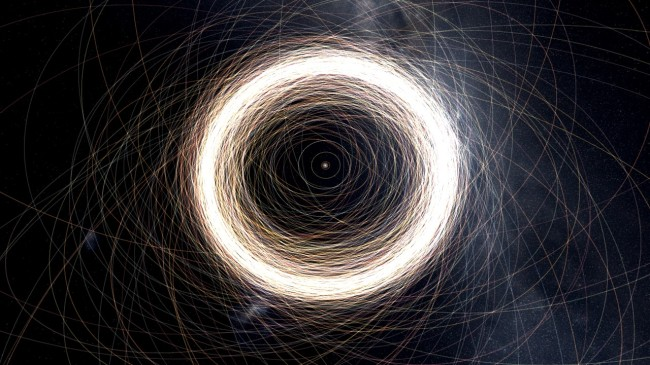
\includegraphics[width=0.85\textwidth]{sandbox2.jpg}
	\caption{An illustration of an orbital timelapse in Universe Sandbox$^2$}
	\cite{nbodypic}
\end{figure} 

\subsection*{Brute-Force algorithm}
The most obvious and most accurate algorithm of solving the N-body simulation is simply a brute-force approach. This algorithm makes sure to compute the forces that are being applied between all pairs of space particles within a given system, thus ensuring scientifically correct movements.

Of course, being a brute-force algorithm, the asymptotic bound on computation time is not very good. Because the algorithm needs to touch all particle pairs during a single iteration of the computation, the time complexity is bounded by $O(n^2)$.

\subsection*{Barnes-Hut algorithm}
A different approach is the Barnes-Hut algorithm. This algorithm is a mere approximation of the N-body simulation problem, so it is best used when computational time is a constraint and the physical accuracy is not as important.

The algorithm divides the whole computation space into quadrant cells. The algorithm then only computes the forces between particles within a single cell, not taking into consideration any other single particles. 

\begin{figure}[ht]
	\centering
	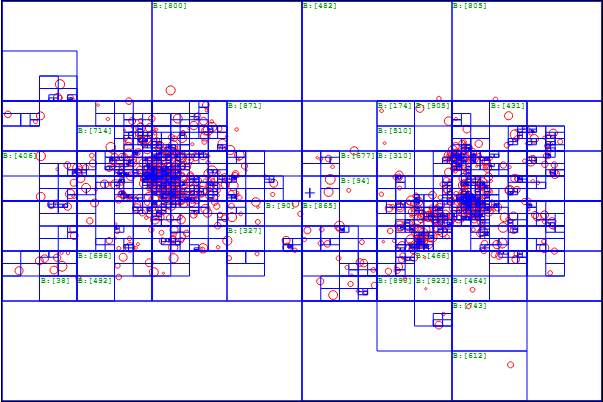
\includegraphics[width=0.75\textwidth]{barneshut.png}
	\caption{An illustration of the Barnes-Hut quadrant division}
	\cite{barnespic}
\end{figure} 

All other cells are then treated as one, massive particle, which has the mass of all particles cells contained within a given cell. The position of this dense particle is centered around the center of mass of all neighboring particles within that cell. Other than this modification, the algorithm still works very similarly to the brute-force algorithm. 

The fact that only a single big particle is used in the computation drastically reduces the number of particle pairs that have to be compared. The time complexity of the Barnes-Hut algorithm is $O(n \cdot logn)$.

It is important the mention the drawbacks of this algorithm. Because of the approximated mass of a majority of particles during a single iteration, the algorithm is not very accurate in the scientific scope. Apparently, the recursive nature of the algorithm also makes it somewhat unsuitable for parallel implementations, meaning that the brute-force algorithm might perform better on a massively multi-threaded machine with reasonable amounts of galactic particles.

I chose to pursue the brute-force algorithm for these reasons. 

\section{Related work in literature}

Typical N-body simulation problems can be traced to the 1960s. The first astrophysical simulation was performed by Sebastian von Hoerner in 1960 for a dynamic system consisting of just 16 particles. \cite{camb_book}

At that time, the lack of computational facilities meant that scientists had to decide between performing fewer interation of the simulation with the highest amount of particles (\textit{N}) possible, or perform a much more in-depth study of smaller systems.\cite{camb_book}

A milestone of $N=100$ bodies was reached by S. J. Aarseth in 1962. Another milestone of $N=500$ for spherical liquid bodies was reached in 1964 by A. Rahman. \cite{history}

Since those times, it can be said that the performance of N-body simulations has been limited by Moore’s law and therefore advancements in moden computer architectures. A significant single-machine speedup was reached with the introduction of multi-core processors. Another fairly large (and recent) leap in computational performance was caused by the spread of graphical processing units (GPUs). Technologies like \textit{OpenCL} and \textit{CUDA} have been extremely helpful in all kinds of topics in the field of scientific computations.

N-body simulations have been at the forefront of high-performance computing in the terms of \textit{FLOP/s} (or floating point operations per second) that they deliver.\cite{history} This is especially true for the brute-force N-body algorithm, as it responds fairly well to parallelization. 

There have been discussions whether the \textit{FLOP/s} metric is even useful in comparing these algorithms, or whether the "amount of science done" should be considered instead. Other strategies, such as the Barnes-Hut algorithm, may be less efficient theoretically, but they can deliver more information in the same amount of computation time.

Nowadays, it is possible to simulate dynamic systems with as many as $10^{11}$ space particles. In 2010, a team of programmers at Nagasaki University in Japan created a parallel implementation of the N-body problem using nVidia’s CUDA technology. When ran on a supercomputer containing a total of 576 \textit{GT200} (Tesla 2.0 architecture) GPUs, they measured a performance of 190.5 \textit{TFLOP/s}. \cite{teraflops}

The theoretical processing power of such a supercomputer should be right around 580 \textit{TFLOP/s}, as one \textit{GT200} chip can produce as many as (depending on core configuration and clock speeds) 1010 \textit{GFLOP/s}.\cite{wikitesla}

The resulting 190.5 \textit{TFLOP/s} is a very respectable number, especially since the code that was used to run the computation used the Barnes-Hut algorithm, instead of the „faster“ (\textit{FLOP/s}-wise) brute-force method.

\section{Methods and facilities to be used}
I will try to create an efficient implementation of the brute-force algorithm with regards to cache-friendliness, then I will parallelize it using OpenMP and possibly CUDA, if time constraints permit. 
I will then measure the computation times on a multitude of different devices:
\begin{itemize}  
\item[-]{a typical personal computer CPU architecture, i.e. Intel’s x86-64. I will use KSU’s Beocat supercomputer to run the tests on this architecture.}
\item[-]{an ARM-architecture based computer. I will use my own OrangePi One micro-computer, which is currently setup as a media center in my home. This micro-computer uses a single Allwinner H3 SoC (system-on-chip) with a quad-core processor and an integrated GPU. The CPU's clock speed is 1200 MHz. I will install a fresh distribution of ARMbian on it and run my tests that way.}
\item[-]{a computer equipped with Intel’s Xeon Phi coprocessor card. I hope to confirm my theoretical knowledge I have about this coprocessor card – that it is extremely suitable for simple, embarrassingly parallel computations and vector computing. I hope to see a massive speedup compared to Intel’s x86-64 architecture. I will run my tests on a Xeon Phi-equipped computer at my home university (CTU in Prague, CZ).}
\item[-]{if time permits, I would like to run a CUDA implementation on a computer equipped with an nVidia graphics processor. I would like to run these benchmarks on nodes that are part of Beocat and have dedicated GPUs just for this purpose.}
\end{itemize}

\section{Breakdown of tasks, time and work schedule}
The first step I will need to take is the implementation of a really simple, unoptimized, sequential N-body simulation algorithm. 

Then I will probably develop some kind of graphical interface just to better understand what exactly is happening during my calculations, and to help me debug the algorithm better. Another good side of this step is that it will probably look cool.

After obtaining a working naive sequential implementation of the project, I will start my work on redesigning the algorithm in a more efficient manner. I will try to maximize the usage of all system resources, which of course includes the usage of a parallel interface.

Next I will modify my code in order to incorporate the OpenMP library into it. I will also use Intel compiler functions to further transform my code to cooperate with the Xeon Phi coprocessor card.

I will also try to create a parallel version of my implementation using nVidia’s CUDA technology.

I will then test and measure running times with a variable amount of cores used for the computation and a variable amount of bodies (particles). I will try to collect a large amount of test data to get a better grasp on the overall performance of the algorithm when used on different machines and chips.

The last step in my course project will be the analysis of data will be gathered. I will try my best to draw conclusions that reflect the test results and explain the differences in performance.

To put my work schedule into perspective, please see the Gantt chart below.

\begin{figure}[ht]
	\centering
	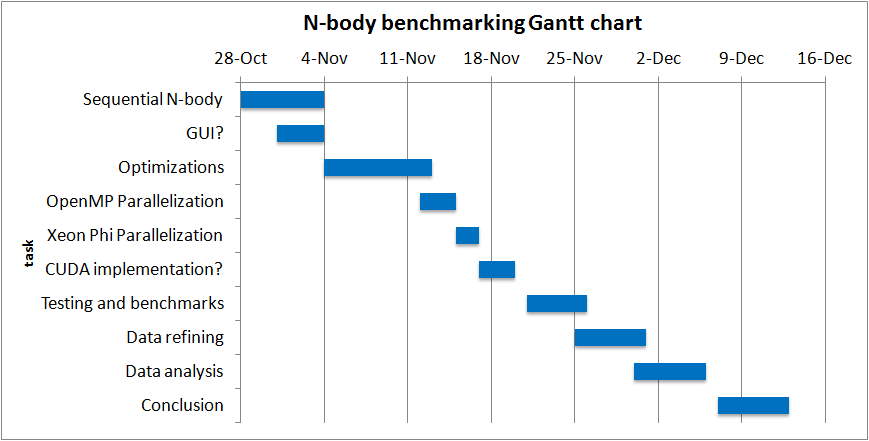
\includegraphics[width=\textwidth]{ganttchart.png}
	\caption{Gantt chart of an estimated project working schedule}
\end{figure} 

\pagebreak
\bibliographystyle{ieeetr}
\bibliography{mybibliographyfile}

\end{document}